% Provenance (never printed): see sources/outline_sources.md (Year 2: sedimentary basins;
% subsidence curves and backstripping; the stretching model). Stretching model after McKenzie
% (1978) as restated by Sheplev and Reverdatto (1998) and coded in pyBacktrack (EarthByte);
% backstripping after pyBacktrack's well module; North Sea after Sclater and Christie (1980);
% Michigan after Sloss (1982) and Crowe et al. (2009); the US Atlantic margin after Schlee et
% al. (1976), Poag (1979) and Lang et al. (2024); the Molasse after the chapter 13 rows.
% Curves and the invented well from figdata/bachelor-2/basins.py; exercise and problem values
% in the Book 4 scratch calculator calc/ch16.py.
\chapter{Sedimentary Basins Compared}\label{ch:b2:basins-compared}

Off the coast of the eastern United States, beneath the continental shelf, the Baltimore
Canyon Trough holds at least \qty{14}{km} of sedimentary rock. A borehole drilled into such a
pile reads its history backwards: each unit it crosses was once the sea floor, at a depth that
fossils and sediments record, and has since been buried and squeezed. The depth of every
dated surface is a point on a curve of sinking. Yet most of the sinking was caused by the
weight of the sediment itself. To learn what made the basin, that weight has to be taken off,
layer by layer. This chapter shows how, and what the result says about the lithosphere.
% ledger: poag79:bct, schlee76:atlantic

\begin{recall}
\textbf{From the Year 1 volume}: sedimentary basin, subsidence and tectonic subsidence,
accommodation, eustasy; compaction, decompaction and Athy's law, the solid thickness of a
layer; the sediment load, which amplifies subsidence by $(\rho_m - \rho_w)/(\rho_m - \rho_s)$;
Airy isostasy; the lithosphere and its geotherm; continental rifts and passive margins.
\textbf{From the physics volumes}: the heat equation and its Fourier solutions.
\textbf{From \cref{ch:b2:alpine-orogen}}: the \omterm{def:b2:alpine-orogen:foreland}{foreland basin}, \omterm{def:b2:alpine-orogen:foreland}{flysch} and \omterm{def:b2:alpine-orogen:foreland}{molasse}.
\end{recall}

\begin{omfigure}
\centering
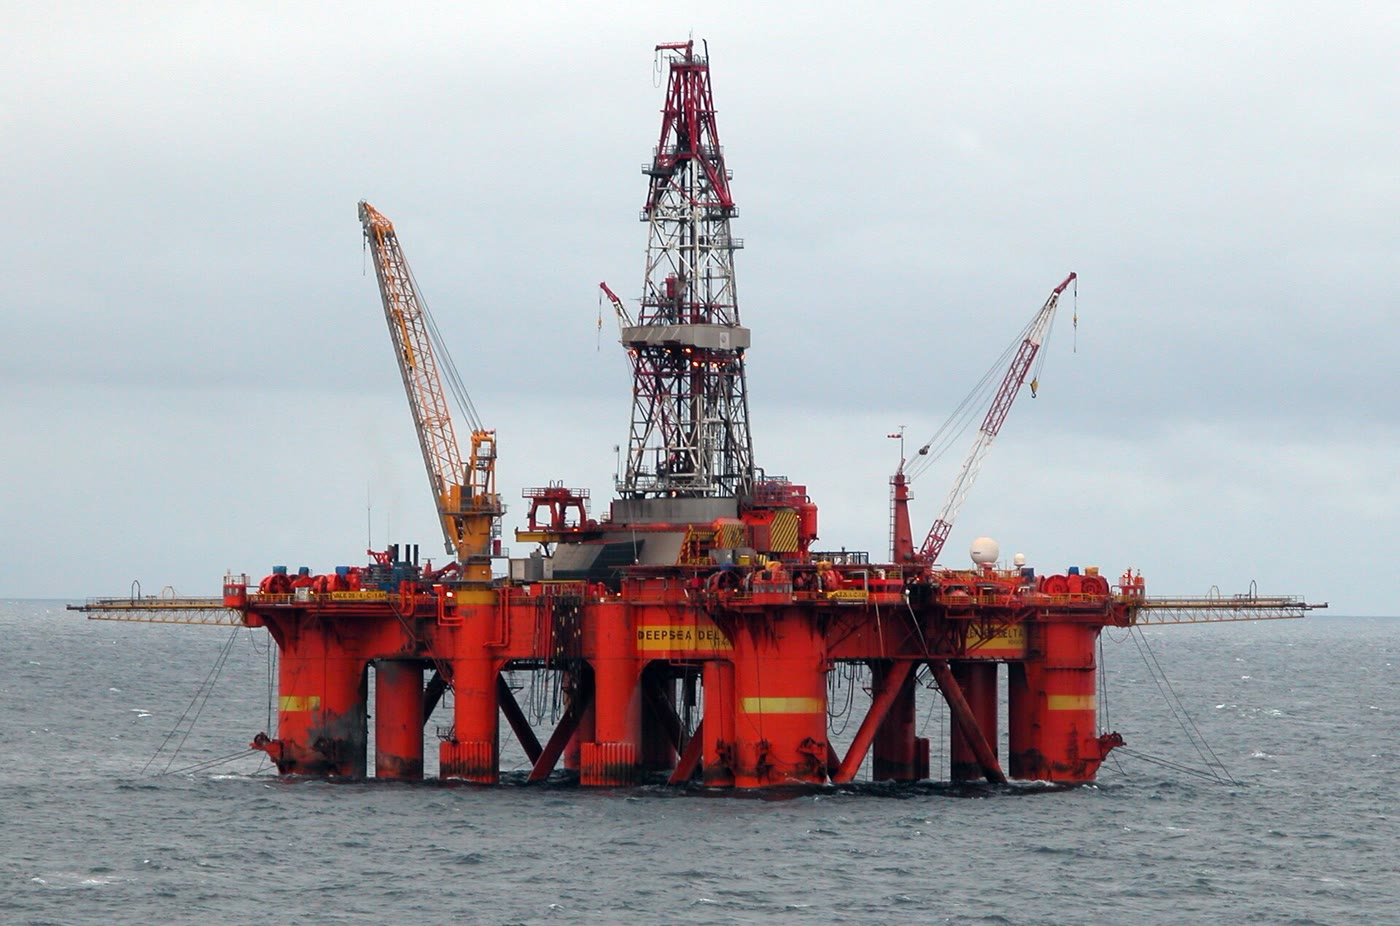
\includegraphics[width=0.66\linewidth]{images/book4/b2-16-drilling-rig.jpg}
\par\smallskip{\small A semi-submersible drilling rig in the North Sea. The boreholes drilled
from such rigs give the thicknesses, ages and rock types from which the subsidence of a basin
is reconstructed. Photograph Erik Christensen, 2005, CC BY-SA 3.0.}
\end{omfigure}

\section{Basins and what makes them sink}\label{sec:b2:basins-compared:types}

The Year 1 volume told basins apart by where they lie. Here they are told apart by what drives
their subsidence.

\begin{definition}[Intracratonic, rift and passive-margin basins]\label{def:b2:basins-compared:types}
An \emph{intracratonic basin}\index{intracratonic basin} is a broad, round or oval basin in the
interior of a continent, far from plate boundaries, that subsides slowly over very long times
without major faulting. A \emph{rift basin}\index{rift basin} is a basin bounded by normal faults
in a continental lithosphere being stretched; its subsidence follows the stretching and then
the cooling of the lithosphere. A \emph{passive-margin basin}\index{passive-margin basin} is the
wedge of sediment, thickening oceanwards, that accumulates on a continental margin after
break-up, over the thinned crust of the old rift.
\end{definition}

The \omterm{def:b2:alpine-orogen:foreland}{foreland basin} of \cref{ch:b2:alpine-orogen} completes the list, and the basins that open
along strike-slip faults are left to the Year 3 volume. Three mechanisms make the floor of a
basin sink:
\begin{itemize}
  \item \emph{mechanical} thinning: when the crust is stretched and thinned by faults, light
        crust is replaced by denser mantle and the surface goes down to restore isostasy;
  \item \emph{thermal} contraction: a lithosphere that has been heated, by stretching or from
        below, cools afterwards, grows denser and sinks, slowly, over tens of millions of years;
  \item \emph{loading}: the weight of a thrust belt, or of the sediment itself, bends the
        lithosphere down; that flexure belongs to the Year 3 volume, and the local, Airy form of
        the sediment load is enough here.
\end{itemize}
\omterm{def:b2:basins-compared:types}{Rift basins} combine the first two, passive margins inherit the second from their rift stage,
\omterm{def:b2:alpine-orogen:foreland}{foreland basins} are made by the third. \omterm{def:b2:basins-compared:types}{Intracratonic basins} are the least understood.

\begin{omfigure}
\centering
\begin{tikzpicture}[x=1cm, y=1cm, font=\scriptsize, line join=round,
  sed/.style={fill=yellow!35, draw=black!60, line width=0.3pt},
  crust/.style={fill=orange!25, draw=black!60, line width=0.3pt},
  mlith/.style={fill=green!12, draw=black!60, line width=0.3pt},
  asth/.style={fill=red!12, draw=black!60, line width=0.3pt},
  sea/.style={fill=blue!8, draw=none},
  ttl/.style={anchor=south west, font=\scriptsize\bfseries}]
% (a) intracratonic
\begin{scope}
\fill[asth] (0,-2.4) rectangle (6.6,-1.6);
\fill[mlith] (0,-1.6) rectangle (6.6,-0.7);
\fill[crust] (0,-0.7) -- (6.6,-0.7) -- (6.6,0) -- (4.9,0) .. controls (4.1,-0.45) and (2.5,-0.45) .. (1.7,0) -- (0,0) -- cycle;
\fill[sed] (1.7,0) .. controls (2.5,-0.45) and (4.1,-0.45) .. (4.9,0) -- cycle;
\draw[black!70] (0,0) -- (6.6,0);
\node[ttl] at (0,0.05) {(a) intracratonic};
\node at (3.3,-1.15) {mantle lithosphere};
\node at (3.3,-2.0) {asthenosphere};
\end{scope}
% (b) rift
\begin{scope}[xshift=7.2cm]
\fill[asth] (0,-2.4) -- (6.6,-2.4) -- (6.6,-1.6) -- (4.5,-1.6) -- (3.3,-1.0) -- (2.1,-1.6) -- (0,-1.6) -- cycle;
\fill[mlith] (0,-1.6) -- (2.1,-1.6) -- (3.3,-1.0) -- (4.5,-1.6) -- (6.6,-1.6) -- (6.6,-0.7) -- (4.4,-0.7) -- (3.3,-0.45) -- (2.2,-0.7) -- (0,-0.7) -- cycle;
\fill[crust] (0,-0.7) -- (2.2,-0.7) -- (3.3,-0.45) -- (4.4,-0.7) -- (6.6,-0.7) -- (6.6,0) -- (4.6,0) -- (4.25,-0.42) -- (3.75,-0.2) -- (3.35,-0.4) -- (2.95,-0.15) -- (2.45,-0.42) -- (2.0,0) -- (0,0) -- cycle;
\fill[sed] (2.0,0) -- (2.45,-0.42) -- (2.95,-0.15) -- (3.35,-0.4) -- (3.75,-0.2) -- (4.25,-0.42) -- (4.6,0) -- cycle;
\draw[thick] (2.0,0) -- (2.5,-0.5) (4.6,0) -- (4.2,-0.5) (2.95,-0.15) -- (3.4,-0.48);
\draw[black!70] (0,0) -- (6.6,0);
\node[ttl] at (0,0.05) {(b) rift};
\node at (1.45,-1.15) {mantle lithosphere};
\node at (5.4,-2.0) {asthenosphere};
\end{scope}
% (c) passive margin
\begin{scope}[yshift=-3.3cm]
\fill[asth] (0,-2.4) -- (6.6,-2.4) -- (6.6,-1.2) -- (0,-1.6) -- cycle;
\fill[mlith] (0,-1.6) -- (6.6,-1.2) -- (6.6,-1.0) -- (4.2,-1.05) -- (2.4,-0.75) -- (0,-0.7) -- cycle;
\fill[crust] (0,-0.7) -- (2.4,-0.75) -- (4.2,-1.05) -- (4.2,-0.85) -- (2.6,-0.25) -- (1.6,0) -- (0,0) -- cycle;
\fill[gray!35, draw=black!60, line width=0.3pt] (4.2,-1.05) -- (6.6,-1.0) -- (6.6,-0.85) -- (4.2,-0.85) -- cycle;
\fill[sed] (1.6,0) -- (2.6,-0.25) -- (4.2,-0.85) -- (6.6,-0.85) -- (6.6,-0.55) -- (3.6,-0.45) -- (2.6,-0.05) -- (2.2,0) -- cycle;
\fill[sea] (2.2,0) -- (6.6,0) -- (6.6,-0.55) -- (3.6,-0.45) -- (2.6,-0.05) -- cycle;
\draw[black!70] (0,0) -- (2.2,0);
\draw[blue!60!black] (2.2,0) -- (6.6,0);
\node[ttl] at (0,0.05) {(c) passive margin};
\node at (5.4,-0.95) {\tiny oceanic crust};
\node at (1.3,-2.0) {asthenosphere};
\node at (1.3,-1.05) {mantle lithosphere};
\end{scope}
% (d) foreland
\begin{scope}[xshift=7.2cm, yshift=-3.3cm]
\fill[asth] (0,-2.4) -- (6.6,-2.4) -- (6.6,-2.0) -- (0,-1.5) -- cycle;
\fill[mlith] (0,-1.5) -- (6.6,-2.0) -- (6.6,-1.2) -- (0,-0.7) -- cycle;
\fill[crust] (0,-0.7) -- (6.6,-1.2) -- (6.6,-0.55) -- (3.6,-0.4) .. controls (2.0,-0.15) .. (0,0) -- cycle;
\fill[sed] (0,0) .. controls (2.0,-0.15) .. (3.6,-0.4) -- (6.6,-0.55) -- (5.0,0) -- cycle;
\fill[crust, fill=orange!45] (5.0,0) -- (6.6,-0.55) -- (6.6,0.6) -- (6.1,0.6) -- cycle;
\draw[thrust fault] (6.6,-0.55) -- (5.0,0);
\draw[black!70] (0,0) -- (5.0,0);
\node[ttl] at (0,0.05) {(d) foreland};
\node[anchor=north east, font=\tiny] at (6.55,0.55) {belt};
\node at (2.2,-1.25) {mantle lithosphere};
\node at (1.5,-2.05) {asthenosphere};
\end{scope}
\end{tikzpicture}
\par\smallskip{\small Four families of basins in schematic sections across the lithosphere (not
to scale; sediment in yellow, continental crust in orange, oceanic crust in grey). The vertical
exaggeration is large: real basins are hundreds of kilometres wide and a few to fifteen
kilometres deep.}
\end{omfigure}

The \omterm{def:b2:basins-compared:types}{rift basins} of the North Sea are the classic case of the first two mechanisms. Grabens
formed there from the Triassic, and the last major stretching lasted from the Middle Jurassic
to the mid-Cretaceous; the faults then fell quiet, and the middle of the basin went on sinking
as a broad saucer, filled by chalks, sandstones and, through most of the Tertiary, shales and
mudstones. Loaded by water alone, its basement would have sunk a further 1100 to
\qty{1400}{m} in the middle and 600 to \qty{700}{m} on the flanks after the faulting had stopped.
% ledger: sc80b4:north-sea

The passive margin of the eastern United States shows the same sinking on a larger scale.
Seismic profiles across the shelf show more than \qty{14}{km} of Mesozoic and younger rock in
the Baltimore Canyon Trough and \qty{8}{km} in the Georges Bank basin, in units that thicken
oceanwards. Its Jurassic depocentres follow the structures of the rift and the zones of its
later thermal subsidence.
% ledger: schlee76:atlantic, lang24:atlantic

The Michigan basin is the type of the \omterm{def:b2:basins-compared:types}{intracratonic basins}. Ovate, some hundreds of thousands
of square kilometres in area, it holds more than \qty{4}{km} of Phanerozoic sediment laid down
in distinct episodes over some 500 million years, with little faulting. Its episodes of faster
subsidence coincide with those of other basins in the interiors of North America and other
continents, which suggests a cause larger than one basin. \omterm{def:b2:basins-compared:backstripping}{Backstripping} more than 57\,000
well logs shows a long-lived, nearly circular pattern of subsidence, which the authors suggest
mantle downwelling could explain, interrupted at the times of two orogenies on the distant
margin of the continent. Why \omterm{def:b2:basins-compared:types}{intracratonic basins} sink is still debated.
% ledger: sloss82:michigan, crowe09:michigan

\section{Subsidence curves}\label{sec:b2:basins-compared:curves}

A well, or a measured section, gives for each unit its present depth, its rock type and its age,
read from fossils or from correlation. With the depth of water in which each unit was laid
down, read from its fossils and sedimentary structures, it gives the history of the basin.

\begin{definition}[Subsidence curve]\label{def:b2:basins-compared:curve}
A \emph{subsidence curve}\index{subsidence curve} of a basin at a site is the graph of the depth
of a reference surface, usually the basement or the base of the oldest unit, below sea level,
against time. The \emph{total} subsidence curve uses the sediment thickness as it was at each
time, plus the water depth; the \emph{tectonic} subsidence curve replaces the sediment by water
and removes its isostatic effect.
\end{definition}

A unit is never as thick in the past as it is today. Buried, it lost porosity; its grains have
not changed, but its water has been squeezed out. The Year 1 volume wrote the porosity at depth
$z$ as Athy's law, $\phi(z) = \phi_0\,e^{-z/c}$, and found the solid thickness of a layer between
$z_1$ and $z_2$,
\[
  T_s = (z_2 - z_1) - \phi_0 c\left(e^{-z_1/c} - e^{-z_2/c}\right),
\]
which stays the same when the layer moves. To \emph{decompact} a unit to a shallower position,
with its top now at $z_1'$, one looks for the base $z_2'$ that holds the same solid thickness. The
equation has no closed solution, but the fixed-point iteration
\[
  z_2' \leftarrow z_1' + T_s + \phi_0 c\left(e^{-z_1'/c} - e^{-z_2'/c}\right)
\]
starting from $z_2' = z_1' + T_s$ converges in a few steps. The mass per unit area of the layer
is that of its grains plus that of its pore water,
\[
  m = \rho_g T_s + \rho_w\,(z_2 - z_1 - T_s),
\]
with $\rho_g$ the density of the grains; dividing the mass of a column by its thickness gives
its mean density $\bar\rho_s$.

For the lithologies used in this chapter, sand, shale, chalk and shaly sand, the table below
gives the constants of Sclater and Christie (1980), as bundled in an open-source program.
Sand keeps its porosity deepest, chalk loses it fastest.
% ledger: pybacktrack:compaction

\begin{center}
\small
\begin{tabular}{lccc}
\hline
lithology & grain density (\unit{kg.m^{-3}}) & surface porosity $\phi_0$ & decay length $c$ (\unit{m}) \\
\hline
sand & 2650 & 0.49 & 3704 \\
shale & 2700 & 0.63 & 1960 \\
chalk & 2710 & 0.70 & 1408 \\
shaly sand & 2680 & 0.56 & 2564 \\
\hline
\end{tabular}
\end{center}

\section{Backstripping}\label{sec:b2:basins-compared:backstripping}

A total \omterm{def:b2:basins-compared:curve}{subsidence curve} mixes two causes: whatever made the basin, and the weight of what
filled it. Separating them is the purpose of the next procedure, the central tool of basin
analysis.

\begin{definition}[Backstripping]\label{def:b2:basins-compared:backstripping}
\emph{Backstripping}\index{backstripping} is the reconstruction of the tectonic subsidence of a
basin through time: the units of a well are removed one by one, from the youngest, the
remaining ones are decompacted at each step, and the isostatic effect of the sediment and water
load is removed to give the depth at which the basement would have stood under water alone.
\end{definition}

The last step is an isostatic balance. The Year 1 volume made it for a basin filled to sea level;
the general case adds the depth of water and the level of the sea.

\begin{proposition}[Airy backstripping]\label{prop:b2:basins-compared:backstrip}
Let a basin hold, at some time, a sediment column of thickness $S$ and mean density
$\bar\rho_s$, under a water depth $W_d$, while the sea stood $\Delta_{SL}$ above its present
level. In local isostasy over a mantle of density $\rho_m$, with water of density $\rho_w$, the
tectonic subsidence at that time, measured from present sea level, is
\[
  Y = S\,\frac{\rho_m - \bar\rho_s}{\rho_m - \rho_w} + W_d
      - \Delta_{SL}\,\frac{\rho_m}{\rho_m - \rho_w}.
\]
\end{proposition}

\begin{proof}
Compare two columns over the same lithosphere, down to a depth of compensation below both. In
the first, water of depth $W_d$ lies over the sediment of thickness $S$; in the second, water
alone fills a basin of depth $Y'$ below the same sea surface. Their masses are equal:
\[
  \rho_w W_d + \bar\rho_s S + \rho_m\,(d - W_d - S) = \rho_w Y' + \rho_m\,(d - Y'),
\]
with $d$ the common depth of the compensation level below the sea surface. Hence
$Y'(\rho_m - \rho_w) = S(\rho_m - \bar\rho_s) + W_d(\rho_m - \rho_w)$, which is the first two
terms. If the sea stood $\Delta_{SL}$ higher than today, that extra water is no part of the
basin's own subsidence: removing it, the water-loaded basement rises by
$\Delta_{SL}\rho_w/(\rho_m - \rho_w)$, and its depth below today's sea level is smaller again by
$\Delta_{SL}$; together, $\Delta_{SL}\,\rho_m/(\rho_m - \rho_w)$.
\end{proof}
% ledger: pybacktrack:backstrip

With $\rho_m = \qty{3330}{kg.m^{-3}}$ and $\rho_w = \qty{1030}{kg.m^{-3}}$, a column of sediment of
mean density \qty{2300}{kg.m^{-3}} counts for $1030/2300 = 0.45$ of its thickness in tectonic
subsidence: more than half of the thickness of a basin's fill is made room for by its own weight.
A sea \qty{100}{m} higher than today lowers the result by \qty{145}{m}. The water depth and the
past sea level are the weakest data: fossils give a range of water depths, often hundreds of
metres wide on the slope, and the tectonic subsidence inherits that range.

\begin{method}[Backstripping a well]\label{met:b2:basins-compared:backstrip}
\begin{enumerate}
  \item List the units from the base, with the present depths of their tops and bases, their
        lithology constants $(\rho_g, \phi_0, c)$, the ages of their tops, and the water depth at
        each of those ages.
  \item Compute the solid thickness $T_s$ of each unit from its present depths.
  \item For the age of the top of unit $k$, remove all the younger units. Put the top of unit
        $k$ at depth zero and decompact it; put each older unit, in turn, under the one above it
        and decompact it.
  \item Add up the thicknesses to give $S$, and the masses to give the mean density
        $\bar\rho_s = \sum m / S$.
  \item Apply \cref{prop:b2:basins-compared:backstrip} to obtain $Y$; the total subsidence is
        $S + W_d$.
  \item Repeat for each age, from the oldest to the present; plot $Y$ and $S + W_d$ against age.
\end{enumerate}
\end{method}

The figure below shows the result for an invented well in a \omterm{def:b2:basins-compared:types}{rift basin}. Four units were cored:
a syn-rift sand laid down while faults were active, between 165 and \qty{150}{Ma}; then a shale,
a chalk and a shaly sand. Today, no decompaction is needed: the basement lies at \qty{6030}{m}
and the column has a mean density of \qty{2358}{kg.m^{-3}}, so that $Y = \qty{2648}{m}$ under
\qty{100}{m} of water. At \qty{150}{Ma}, the sand alone, decompacted at the surface, was
\qty{2239}{m} thick, with a mean density of \qty{2055}{kg.m^{-3}}: under \qty{200}{m} of water,
$Y = \qty{1441}{m}$. The total subsidence is
more than twice the tectonic one, and the tectonic curve shows a fast first stage, then a
slowing sinking: the shape of a rift.
% values (script): figdata/bachelor-2/basins.py part numbers (S_150 2239.5, rho_0 2357.9, Y_0 2648.7, Y_150 1442.1); printed from the rounded chain of calc/ch16.py (rho 2358 -> 2648; T 2239, rho 2055 -> 1441), as in the problem

\begin{omfigure}
\centering
% figdata/bachelor-2/basins.py parts stages and fit (invented well)
\begin{tikzpicture}
\begin{axis}[width=0.8\linewidth, height=6.0cm, x dir=reverse, y dir=reverse, xmin=0, xmax=170,
  ymin=0, ymax=6500, xlabel={age (\unit{Ma})}, ylabel={depth below sea level (\unit{m})},
  tick label style={font=\scriptsize}, label style={font=\small}, xtick={0,25,...,175},
  xtick pos=bottom, ytick pos=left,
  legend style={at={(0.5,1.04)}, anchor=south, draw=none, font=\scriptsize, legend columns=3,
  /tikz/every even column/.append style={column sep=8pt}}]
\addplot[omThm, line width=1pt, mark=*, mark size=1.6pt] table[x=age_Ma, y=total_m]
  {figdata/out/bachelor-2-basins-stages.dat};
\addlegendentry{total subsidence $S + W_d$}
\addplot[blue!70!black, line width=1pt, mark=square*, mark size=1.6pt] table[x=age_Ma, y=Y_m]
  {figdata/out/bachelor-2-basins-stages.dat};
\addlegendentry{tectonic subsidence $Y$}
\addplot[black!70, dashed, line width=0.8pt] table[x=age_Ma, y=Y_m]
  {figdata/out/bachelor-2-basins-fit.dat};
\addlegendentry{stretching model, $\beta = 1.50$}
\node[font=\scriptsize, anchor=south west] at (axis cs:149,1500) {end of rifting};
\end{axis}
\end{tikzpicture}
\par\smallskip{\small \omterm{def:b2:basins-compared:backstripping}{Backstripping} of an invented well with four units (data in the weekend
problem): basement depth with the sediment as it was at each time, and tectonic subsidence,
with the curve of the \omterm{def:b2:basins-compared:stretching}{stretching model} fitted to the subsidence at the end of rifting
(\cref{sec:b2:basins-compared:stretching}).}
\end{omfigure}

\begin{omfigure}
\centering
\begin{tikzpicture}[x=1cm, y=0.1cm, font=\scriptsize, line join=round,
  u/.style={draw=black!60, line width=0.3pt}]
% today
\begin{scope}
\fill[blue!8] (0,0) rectangle (1.6,-1.0);
\fill[u, fill=yellow!25] (0,-1.0) rectangle (1.6,-18.0);
\fill[u, fill=green!18] (0,-18.0) rectangle (1.6,-34.1);
\fill[u, fill=gray!25] (0,-34.1) rectangle (1.6,-45.2);
\fill[u, fill=yellow!55] (0,-45.2) rectangle (1.6,-61.3);
\draw[black!70] (0,-61.3) -- (1.6,-61.3);
\node[anchor=south] at (0.8,0.1) {today};
\node at (0.8,-9.5) {shaly sand};
\node at (0.8,-26) {chalk};
\node at (0.8,-39.6) {shale};
\node at (0.8,-53.2) {sand};
\node[anchor=north] at (0.8,-61.5) {\qty{6130}{m}};
\end{scope}
% at 150 Ma
\begin{scope}[xshift=3.0cm]
\fill[blue!8] (0,0) rectangle (1.6,-2.0);
\fill[u, fill=yellow!55] (0,-2.0) rectangle (1.6,-24.39);
\draw[black!70] (0,-24.4) -- (1.6,-24.4);
\node[anchor=south] at (0.8,0.1) {\qty{150}{Ma}};
\node at (0.8,-13.2) {sand};
\node[anchor=north] at (0.8,-24.6) {\qty{2439}{m}};
\end{scope}
\draw[-{Latex}, thick] (4.9,-12) -- (6.1,-12) node[midway, above] {unload};
% water loaded
\begin{scope}[xshift=6.3cm]
\fill[blue!20] (0,0) rectangle (1.6,-14.4);
\draw[black!70] (0,-14.4) -- (1.6,-14.4);
\node[anchor=south] at (0.8,0.1) {water only};
\node at (0.8,-7.2) {water};
\node[anchor=north] at (0.8,-14.6) {$Y = \qty{1441}{m}$};
\end{scope}
\draw[black!40, dashed] (-0.3,0) -- (8.2,0);
\node[anchor=west] at (8.2,0) {sea level};
\end{tikzpicture}
\par\smallskip{\small \omterm{def:b2:basins-compared:backstripping}{Backstripping} the invented well at \qty{150}{Ma} (depths to scale): the
four units today; the sand alone at the end of rifting, decompacted at the surface under
\qty{200}{m} of water; the same lithosphere loaded by water alone, whose basement stands
higher because water is lighter than sediment.}
\end{omfigure}

\section{The stretching model}\label{sec:b2:basins-compared:stretching}

Why does a \omterm{def:b2:basins-compared:types}{rift basin} sink first fast and then slowly? In 1978 D. McKenzie proposed a model so
simple that its parameters can be fitted to a single well.

\begin{definition}[Stretching model; stretching factor; syn-rift and post-rift subsidence]\label{def:b2:basins-compared:stretching}
The \emph{stretching model}\index{stretching model} of a basin represents rifting as an
instantaneous, uniform stretching of the whole lithosphere by pure shear: crust and mantle
lithosphere are thinned by the same factor, and hot asthenosphere rises passively to fill the
space, after which the lithosphere cools. The \emph{stretching factor}\index{stretching factor}
$\beta$ is the ratio of the width of the stretched region after stretching to its width before,
equal to the ratio of the initial to the final thickness of the crust. The subsidence produced
during stretching is the \emph{syn-rift subsidence}\index{syn-rift subsidence}; that produced
afterwards by the cooling of the lithosphere is the \emph{post-rift
subsidence}\index{post-rift subsidence}, or thermal subsidence.
\end{definition}

Stretching in nature takes a finite time, millions of years. Later versions of the model let it
last, but as long as it is not too slow the simple instantaneous version gives the subsidence
roughly but correctly, since after the stretching the cooling proceeds in much the same way.
% ledger: sheplev98:model

\begin{omfigure}
\centering
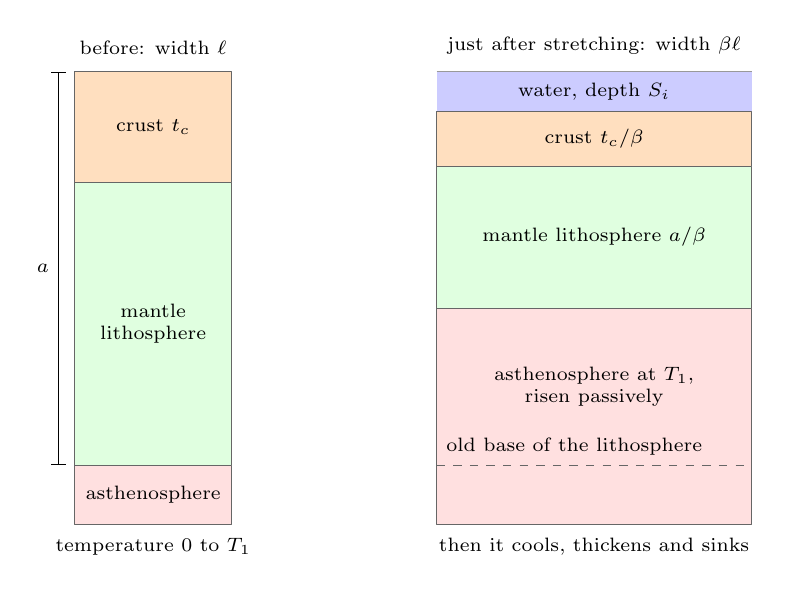
\begin{tikzpicture}[x=0.5cm, y=0.5cm, font=\scriptsize, line join=round]
% before
\begin{scope}
\fill[orange!25, draw=black!60, line width=0.3pt] (0,0) rectangle (4,-2.8);
\fill[green!12, draw=black!60, line width=0.3pt] (0,-2.8) rectangle (4,-10);
\fill[red!12, draw=black!60, line width=0.3pt] (0,-10) rectangle (4,-11.5);
\node at (2,-1.4) {crust $t_c$};
\node[align=center] at (2,-6.4) {mantle\\lithosphere};
\node at (2,-10.75) {asthenosphere};
\draw[|-|] (-0.4,0) -- (-0.4,-10) node[midway, left] {$a$};
\node[anchor=south] at (2,0.2) {before: width $\ell$};
\node[anchor=north] at (2,-11.6) {temperature $0$ to $T_1$};
\end{scope}
% after
\begin{scope}[xshift=4.6cm]
\fill[blue!20] (0,0) rectangle (8,-1.0);
\fill[orange!25, draw=black!60, line width=0.3pt] (0,-1.0) rectangle (8,-2.4);
\fill[green!12, draw=black!60, line width=0.3pt] (0,-2.4) rectangle (8,-6.0);
\fill[red!12, draw=black!60, line width=0.3pt] (0,-6.0) rectangle (8,-11.5);
\draw[black!60, dashed] (0,-10) -- (8,-10);
\node at (4,-0.5) {water, depth $S_i$};
\node at (4,-1.7) {crust $t_c/\beta$};
\node at (4,-4.2) {mantle lithosphere $a/\beta$};
\node[align=center] at (4,-8.0) {asthenosphere at $T_1$,\\risen passively};
\node[anchor=south west] at (0,-10) {old base of the lithosphere};
\node[anchor=south] at (4,0.2) {just after stretching: width $\beta\ell$};
\node[anchor=north] at (4,-11.6) {then it cools, thickens and sinks};
\draw[black!40] (0,0) -- (8,0);
\end{scope}
\end{tikzpicture}
\par\smallskip{\small The \omterm{def:b2:basins-compared:stretching}{stretching model} (not to scale): a lithosphere of thickness $a$ with a
crust $t_c$ is stretched to $\beta$ times its width; crust and mantle lithosphere thin by
$\beta$, the asthenosphere rises, and the surface sinks by the \omterm{def:b2:basins-compared:stretching}{syn-rift subsidence} $S_i$ under
water. Here $\beta = 2$.}
\end{omfigure}

\begin{proposition}[Subsidence in the stretching model]\label{prop:b2:basins-compared:stretching}
Let a lithosphere of thickness $a$, with a crust of thickness $t_c$, have a linear geotherm from
$0$ at the surface to the temperature $T_1$ of the asthenosphere at its base; let crust and mantle
have densities $\rho_c(1 - \alpha T)$ and $\rho_m(1 - \alpha T)$, with $\alpha$ the thermal
expansion coefficient. If it is stretched instantaneously by $\beta$ and the basin filled with
water of density $\rho_w$:
\begin{enumerate}
  \item the \omterm{def:b2:basins-compared:stretching}{syn-rift subsidence} is
  \[
    S_i = \frac{a\left(1 - \dfrac{1}{\beta}\right)\left[(\rho_m - \rho_c)\dfrac{t_c}{a}
          \left(1 - \dfrac{\alpha T_1 t_c}{2a}\right) - \dfrac{\alpha T_1 \rho_m}{2}\right]}
          {\rho_m(1 - \alpha T_1) - \rho_w};
  \]
  \item the \omterm{def:b2:basins-compared:stretching}{post-rift subsidence}, a time $t$ after stretching, is, to the first term of a series,
  \[
    S_t = E_0\,\frac{\beta}{\pi}\sin\frac{\pi}{\beta}\left(1 - e^{-t/\tau}\right),\qquad
    E_0 = \frac{4a\rho_m\alpha T_1}{\pi^2(\rho_m - \rho_w)},\qquad
    \tau = \frac{a^2}{\pi^2\kappa},
  \]
  where $\kappa$ is the thermal diffusivity and $\tau$ is the \emph{thermal time
  constant}\index{thermal time constant} of the lithosphere.
\end{enumerate}
\end{proposition}
% ledger: pybacktrack:rifting

\begin{proof}
(1) Compare the column before stretching with the column just after, down to the old base of
the lithosphere, at depth $a$ below the surface before stretching. Before, the crust of
thickness $t_c$ and the mantle lithosphere are at temperatures $T = T_1 z/a$; after, both are
thinner by $\beta$ and their temperatures run from $0$ to $T_1$ over $a/\beta$, so that a point
at depth $z'$ below the base of the water has $T = T_1\beta z'/a$; beneath, the asthenosphere at
$T_1$ has density $\rho_m(1 - \alpha T_1)$; above, water fills the depth $S_i$. The mass of a
layer of density $\rho(1 - \alpha T)$ in which $T$ grows linearly from $T_a$ to $T_b$ is
$\rho\,h\,(1 - \alpha(T_a + T_b)/2)$. Before, the column holds
\[
  \rho_c t_c\left(1 - \frac{\alpha T_1 t_c}{2a}\right)
  + \rho_m (a - t_c)\left(1 - \frac{\alpha T_1 (a + t_c)}{2a}\right);
\]
after, it holds the water, the thinned crust and mantle lithosphere, and the asthenosphere that
fills the rest of the depth $a$:
\[
  \rho_w S_i + \frac{\rho_c t_c}{\beta}\left(1 - \frac{\alpha T_1 t_c}{2a}\right)
  + \frac{\rho_m (a - t_c)}{\beta}\left(1 - \frac{\alpha T_1 (a + t_c)}{2a}\right)
  + \rho_m(1 - \alpha T_1)\left(a - S_i - \frac{a}{\beta}\right).
\]
Isostasy makes the two equal. Collecting the terms in $S_i$ on one side and the factor
$(1 - 1/\beta)$ on the other, and expanding, gives the formula; the algebra is
\cref{exo:b2:basins-compared:11}.

(2) After stretching, the plate cools by conduction between a surface held at $0$ and a base held
at $T_1$, towards the linear profile it started from. The excess temperature solves the heat
equation with zero values at top and base, and so is a sum of terms
$b_n\sin(n\pi z/a)\,e^{-n^2\kappa\pi^2 t/a^2}$; each cools with its own time, $\tau/n^2$. The
heat lost makes the column contract by $\alpha\int \Delta T\,\mathrm{d}z$, and the extra water
that fills the space sinks it further by the factor $\rho_m/(\rho_m - \rho_w)$. Only odd terms
contribute; keeping the first one, whose coefficient is computed from the initial profile, gives
the expression. The others cool nine or more times faster, and after about ten million years
they shift the subsidence by a nearly constant amount, less than \qty{100}{m} for $\beta$ from
1.2 to 4 with the values below.
\end{proof}
% values (script): basins.thermal_series vs basins.thermal, tested in tests/bachelor-2/test_basins.py

The parameters of McKenzie's paper are $a = \qty{125}{km}$, $T_1 = \qty{1333}{\celsius}$,
$\alpha = \qty{3.28e-5}{K^{-1}}$, $\kappa = \qty{8e-7}{m^2.s^{-1}}$, $\rho_m =
\qty{3330}{kg.m^{-3}}$ (at \qty{0}{\celsius}), $\rho_c = \qty{2800}{kg.m^{-3}}$; with sea water at
\qty{1030}{kg.m^{-3}} they give $\tau = \qty{62.7}{Myr}$ and $E_0 = \qty{3207}{m}$. With a crust of
\qty{35}{km}, the \omterm{def:b2:basins-compared:stretching}{syn-rift subsidence} is $S_i = \qty{4334}{m} \times (1 - 1/\beta)$.
% ledger: sheplev98:parameters, pybacktrack:rifting
% values (script): tau_Myr 62.7, E0_m 3206.9, Si_max_m 4333.8

\begin{omfigure}
\centering
% figdata/bachelor-2/basins.py part curves
\begin{tikzpicture}
\begin{axis}[width=0.8\linewidth, height=6.2cm, y dir=reverse, xmin=0, xmax=200, ymin=0,
  ymax=6500, xlabel={time after stretching (\unit{Myr})},
  ylabel={tectonic subsidence (\unit{m})}, tick label style={font=\scriptsize},
  label style={font=\small}, xtick pos=bottom, ytick pos=left]
\addplot[black!45, line width=1pt] table[x=t_Myr, y=b1.2] {figdata/out/bachelor-2-basins-curves.dat};
\addplot[blue!70!black, line width=1pt] table[x=t_Myr, y=b1.5] {figdata/out/bachelor-2-basins-curves.dat};
\addplot[omThm, line width=1pt] table[x=t_Myr, y=b2] {figdata/out/bachelor-2-basins-curves.dat};
\addplot[orange!80!black, line width=1pt] table[x=t_Myr, y=b4] {figdata/out/bachelor-2-basins-curves.dat};
\node[font=\scriptsize, anchor=south west, inner sep=1pt] at (axis cs:150,1225) {$\beta = 1.2$};
\node[font=\scriptsize, anchor=south west, inner sep=1pt] at (axis cs:150,2595) {$\beta = 1.5$};
\node[font=\scriptsize, anchor=south west, inner sep=1pt] at (axis cs:150,3965) {$\beta = 2$};
\node[font=\scriptsize, anchor=south west, inner sep=1pt] at (axis cs:150,5815) {$\beta = 4$};
\draw[black!40, dashed] (axis cs:62.7,0) -- (axis cs:62.7,6500);
\node[font=\scriptsize, anchor=north west] at (axis cs:63,150) {$t = \tau$};
\end{axis}
\end{tikzpicture}
\par\smallskip{\small Water-loaded subsidence of the \omterm{def:b2:basins-compared:stretching}{stretching model} for four \omterm{def:b2:basins-compared:stretching}{stretching
factors}, with a \qty{35}{km} crust and the parameters of the text: the syn-rift step at
$t = 0$, then the post-rift curve, which has reached \qty{63}{\percent} of its final value at
$t = \tau$.}
\end{omfigure}

Three features of the model carry to real basins.
\begin{itemize}
  \item The syn-rift step grows with $\beta$, and so does the \omterm{def:b2:basins-compared:stretching}{post-rift subsidence}; but their
        ratio changes little, so that both parts point to the same $\beta$ if the model holds.
  \item The time scale of the \omterm{def:b2:basins-compared:stretching}{post-rift subsidence} does not depend on $\beta$: it is set by the
        thickness of the lithosphere alone. After $\tau$, \qty{63}{\percent} of the thermal
        subsidence is done; after $3\tau$, about \qty{95}{\percent}. A rift that stopped two
        hundred million years ago hardly sinks any more.
  \item The syn-rift term is a competition between the light crust thinned, which makes the
        surface sink, and the hot asthenosphere risen, which buoys it up. With a thin crust the
        second wins and stretching raises the surface (\cref{exo:b2:basins-compared:10}).
\end{itemize}

To fit a well, the tectonic subsidence at the end of rifting gives $S_i$, hence
$\beta = 1/(1 - S_i/\qty{4334}{m})$ for a \qty{35}{km} crust; the post-rift curve is then predicted
and compared with the rest of the backstripped points. In the invented well, $S_i = \qty{1441}{m}$
gives $\beta = 1.50$, and the curve passes within a few metres of the later points (figure in
\cref{sec:b2:basins-compared:backstripping}). Real basins are rarely so obliging. In the
central North Sea, stretching of 50 to \qty{100}{\percent} in the middle, $\beta$ from 1.5 to 2,
reproduces the amplitude and rate of the \omterm{def:b2:basins-compared:stretching}{post-rift subsidence}. On the margin of the eastern
United States, only one segment, the Long Island Platform, has an early post-rift fill as thick
as uniform stretching predicts; in the Georges Bank Basin and the Baltimore Canyon Trough the
fill is 1.5 to 3 times thicker, and other causes must be at work.
% ledger: sc80b4:north-sea, lang24:atlantic

\section{Basins compared}\label{sec:b2:basins-compared:compared}

The table below gathers the four families. The curves differ in shape and in time scale, and a
\omterm{def:b2:basins-compared:curve}{subsidence curve} is often the first clue to the nature of a basin buried under younger rocks.

\begin{center}
\small
\begin{tabular}{>{\raggedright\arraybackslash}p{0.13\linewidth}>{\raggedright\arraybackslash}p{0.19\linewidth}>{\raggedright\arraybackslash}p{0.26\linewidth}>{\raggedright\arraybackslash}p{0.29\linewidth}}
\hline
basin & example & thickness and duration & shape of the tectonic \omterm{def:b2:basins-compared:curve}{subsidence curve} \\
\hline
rift & central North Sea & grabens from the Triassic; last stretching Middle Jurassic to
mid-Cretaceous; 1.1 to \qty{1.4}{km} of water-loaded post-rift sinking & a fast syn-rift step,
then an exponential slowing with $\tau$ of tens of Myr \\
passive margin & Baltimore Canyon Trough & more than \qty{14}{km} since the Jurassic & as a
rift, with a large post-rift part; the fill thickens oceanwards \\
foreland & North Alpine \omterm{def:b2:alpine-orogen:foreland}{Molasse} & more than \qty{4}{km} at the thrust front, late Eocene to
late Miocene & deepest against the belt and migrating with it; its inner part finally
overridden by the thrusts \\
intracratonic & Michigan & more than \qty{4}{km} in episodes over some 500 Myr & slow, with
episodes of faster sinking shared by distant basins \\
\hline
\end{tabular}
\end{center}
% ledger: sc80b4:north-sea, schlee76:atlantic, poag79:bct, krenmayr99:molasse, schmid04:foreland, sloss82:michigan

A \omterm{def:b2:alpine-orogen:foreland}{foreland basin} sinks under a load that moves towards it: the basin migrates with the belt,
the Alpine one by at least \qty{210}{km} over the European craton, and its inner part is
finally overridden and carried by the thrusts, as the Subalpine \omterm{def:b2:alpine-orogen:foreland}{Molasse} was in
\cref{ch:b2:alpine-orogen}. A rift slows down as it cools, whatever
its stretching. An \omterm{def:b2:basins-compared:types}{intracratonic basin} sinks slowly and long, in pulses; neither stretching
nor a load explains it well, which is why it remains a research question.
% ledger: schmid04:foreland, sinclair97:trinity, krenmayr99:molasse

\begin{inthelab}[Subsidence analysis]
Basin analysts do the work of the method box with programs. One open-source program, for
instance, reads a drill site as a list of units with their ages, depths and lithologies, and a
table of lithologies with their grain density, surface porosity and decay length. Its
\omterm{def:b2:basins-compared:backstripping}{backstripping} module decompacts the units and returns the tectonic subsidence at each age;
since a palaeo water depth is known only as a range, the user gives a minimum and a maximum and
the program returns the two subsidences and their mean. A second module works the other way:
from a model of tectonic subsidence it predicts the water depths of the past, which can be
checked against the fossils. Analysts then fit \omterm{def:b2:basins-compared:stretching}{stretching factors}, test sea-level curves, and
map the subsidence of a whole basin from hundreds or thousands of wells.
\end{inthelab}
% ledger: pybacktrack:modules, crowe09:michigan

\section*{Exercises}\label{sec:b2:basins-compared:exercises}

Data for the exercises, unless stated otherwise: $\rho_m = \qty{3330}{kg.m^{-3}}$, $\rho_c =
\qty{2800}{kg.m^{-3}}$, $\rho_w = \qty{1030}{kg.m^{-3}}$; \omterm{def:b2:basins-compared:stretching}{stretching model} with $a =
\qty{125}{km}$, $T_1 = \qty{1333}{\celsius}$, $\alpha = \qty{3.28e-5}{K^{-1}}$, $\kappa =
\qty{8e-7}{m^2.s^{-1}}$, $\tau = \qty{62.7}{Myr}$, $E_0 = \qty{3207}{m}$; a \qty{35}{km} crust
gives $S_i = \qty{4334}{m}\times(1 - 1/\beta)$; lithology constants in the table of
\cref{sec:b2:basins-compared:curves}.

\begin{exercise}[$\star$]\label{exo:b2:basins-compared:1}
Name the family of each basin and the main cause of its subsidence: (a) the Michigan basin;
(b) the central North Sea; (c) the Baltimore Canyon Trough; (d) the North Alpine \omterm{def:b2:alpine-orogen:foreland}{Molasse};
(e) the Indo-Gangetic plain in front of the Himalaya.
\end{exercise}

\begin{exercise}[$\star$]\label{exo:b2:basins-compared:2}
A basin holds \qty{3.0}{km} of sediment of mean density \qty{2300}{kg.m^{-3}}. (a) Find its
tectonic subsidence if the sediment reaches sea level. (b) And if \qty{200}{m} of water lie on
top? (c) What fraction of the thickness of the fill is due to the load of the fill itself?
\end{exercise}

\begin{exercise}[$\star$]\label{exo:b2:basins-compared:3}
Seismic refraction shows that a \qty{35}{km} crust has been thinned to \qty{25}{km} in a rift.
(a) What is $\beta$? (b) How thick is the lithosphere just after stretching? (c) What is the
\omterm{def:b2:basins-compared:stretching}{syn-rift subsidence} under water?
\end{exercise}

\begin{exercise}[$\star$]\label{exo:b2:basins-compared:4}
(a) Check that $\tau = \qty{62.7}{Myr}$ ($1~\text{Myr} = \qty{3.156e13}{s}$). (b) Some programs
use $\kappa = \qty{1e-6}{m^2.s^{-1}}$: what is $\tau$ then? (c) What would it be for a
lithosphere \qty{100}{km} thick, with $\kappa = \qty{8e-7}{m^2.s^{-1}}$? (d) What fraction of
the \omterm{def:b2:basins-compared:stretching}{post-rift subsidence} is done after $\tau$, and after $3\tau$?
\end{exercise}

\begin{exercise}[$\star\star$]\label{exo:b2:basins-compared:5}
A shale unit lies today between \qty{1000}{m} and \qty{2000}{m}. (a) Find its porosity at the
top and at the base. (b) Find its solid thickness. (c) Find its mass per unit area and its mean
density, the pores being full of water.
\end{exercise}

\begin{exercise}[$\star\star$]\label{exo:b2:basins-compared:6}
The shale of \cref{exo:b2:basins-compared:5} is brought back to the surface. (a) Iterate the
decompaction formula from $z_2' = T_s$ until it changes by less than \qty{1}{m}. (b) What is
its mean density at the surface? (c) By how much was it thicker?
\end{exercise}

\begin{exercise}[$\star\star$]\label{exo:b2:basins-compared:7}
In the central North Sea, the water-loaded basement sank 1100 to \qty{1400}{m} after the
stretching that ended in the mid-Cretaceous, about \qty{100}{Myr} ago. (a) What \omterm{def:b2:basins-compared:stretching}{post-rift
subsidence} does the model give after \qty{100}{Myr} for $\beta = 1.5$ and $\beta = 2$? (b) Do
those values bracket the observation? (c) For which $\beta$ does the model give \qty{1250}{m}?
Use $\frac{\beta}{\pi}\sin\frac{\pi}{\beta} = 0.4705$ for $\beta = 1.6$ and $0.5204$ for $\beta
= 1.7$ and interpolate.
\end{exercise}

\begin{exercise}[$\star\star$]\label{exo:b2:basins-compared:8}
The syn-rift basin of a \omterm{def:b2:basins-compared:stretching}{stretching model} is filled not with water but with sediment of density
\qty{2300}{kg.m^{-3}}. (a) In the formula for $S_i$, what changes? (b) Compute the sediment-loaded
$S_i$ for $\beta = 1.5$ with a \qty{35}{km} crust, given that the numerator of the formula is
$a(1 - 1/\beta)\times\qty{74.69}{kg.m^{-3}}$ and that $\rho_m(1 - \alpha T_1) =
\qty{3184.4}{kg.m^{-3}}$. (c) Compare with the water-loaded value.
\end{exercise}

\begin{exercise}[$\star\star$]\label{exo:b2:basins-compared:9}
A backstripped well gives $Y = \qty{2171}{m}$ at \qty{100}{Ma}, assuming today's sea level. (a)
If the sea then stood \qty{100}{m} higher, what is $Y$? (b) If the fossils give a water depth
between 100 and \qty{500}{m} instead of \qty{300}{m}, what range of $Y$ follows? (c) Which of the
two uncertainties is the larger?
\end{exercise}

\begin{exercise}[$\star\star\star$]\label{exo:b2:basins-compared:10}
(a) Show from \cref{prop:b2:basins-compared:stretching} that stretching makes the surface rise
instead of sink when $(\rho_m - \rho_c)\frac{t_c}{a}\left(1 - \frac{\alpha T_1 t_c}{2a}\right) <
\frac{\alpha T_1\rho_m}{2}$. (b) Neglecting the small term $\alpha T_1 t_c/(2a)$, find the
critical crustal thickness. (c) Refine it with one iteration. (d) Where on Earth would you look
for rifts that rise as they open?
\end{exercise}

\begin{exercise}[$\star\star\star$]\label{exo:b2:basins-compared:11}
(a) Write the isostatic balance of the proof of \cref{prop:b2:basins-compared:stretching}, part
(1), and derive the formula for $S_i$. (b) Show that the exact final \omterm{def:b2:basins-compared:stretching}{post-rift subsidence}, when
the plate has returned to its linear geotherm, is $\alpha\rho_m T_1 a(1 - 1/\beta)/(2(\rho_m -
\rho_w))$. (c) Compute it for $\beta = 2$ and compare it with the final value of the
first-term formula.
\end{exercise}

\begin{exercise}[$\star\star\star$]\label{exo:b2:basins-compared:12}
A passive margin was stretched by $\beta = 2$ and has been cooling for \qty{150}{Myr}; the
basin has stayed full of sediment of mean density \qty{2400}{kg.m^{-3}} up to sea level.
(a) Find the water-loaded \omterm{def:b2:basins-compared:stretching}{post-rift subsidence}. (b) How thick is the post-rift sediment?
(c) In the Baltimore Canyon Trough the early post-rift fill is 1.5 to 3 times thicker than
uniform stretching predicts: what thickness would that mean here? (d) Suggest causes.
\end{exercise}

\begin{problem}[{Weekend problem --- Backstripping a well}]\label{pb:b2:basins-compared:1}
In the invented Kestrel Basin, a well cored four units. From the base: a sand laid down during
rifting, from 165 to \qty{150}{Ma}, today between \qty{4420}{m} and \qty{6030}{m}; a shale, 150
to \qty{100}{Ma}, between \qty{3310}{m} and \qty{4420}{m}; a chalk, 100 to \qty{60}{Ma}, between
\qty{1700}{m} and \qty{3310}{m}; a shaly sand, \qty{60}{Ma} to today, between \qty{0}{m} and
\qty{1700}{m} below the sea floor. Fossils give the water depth at the top of each unit when it
was laid down: \qty{200}{m} at \qty{150}{Ma}, \qty{300}{m} at \qty{100}{Ma}, \qty{150}{m} at
\qty{60}{Ma}; today it is \qty{100}{m}. Use the lithology table of the chapter, $\rho_m =
\qty{3330}{kg.m^{-3}}$ and $\rho_w = \qty{1030}{kg.m^{-3}}$ for both sea and pore water, sea level
as today, and the \omterm{def:b2:basins-compared:stretching}{stretching model} of the chapter with a \qty{35}{km} crust. Depths are rounded to
the metre.

\noindent\textbf{Part I --- Compaction.}
\begin{enumerate}
  \item Find the porosity of the sand at its top and at its base today.
  \item Find the solid thickness of the sand.
  \item The solid thicknesses of the shale, chalk and shaly sand are \qty{1011}{m},
        \qty{1409}{m} and \qty{1004}{m}. Check one of them.
  \item Find the mass per unit area of each unit today, then the mean density of the whole
        column.
  \item At \qty{150}{Ma} the sand lay at the sea floor. Decompact it: iterate from $z_2' =
        T_s$ until the change is less than \qty{1}{m}.
  \item Find the mean density of the decompacted sand.
\end{enumerate}

\noindent\textbf{Part II --- Backstripping.}
\begin{enumerate}[resume]
  \item Find the tectonic subsidence $Y$ at \qty{150}{Ma}.
  \item Find the tectonic subsidence today. Why is no decompaction needed?
  \item A program gives $Y = \qty{2171}{m}$ at \qty{100}{Ma} and $Y = \qty{2453}{m}$ at
        \qty{60}{Ma}. Compute the mean rate of tectonic subsidence in each of the three
        intervals since \qty{150}{Ma}.
  \item Find the total subsidence today and compare it with the tectonic subsidence.
  \item What fraction of the depth of the basement today is due to the load of the sediment?
  \item If the sea at \qty{100}{Ma} had stood \qty{100}{m} higher than today, what would $Y$
        have been then?
\end{enumerate}

\noindent\textbf{Part III --- Fitting the stretching model.} Rifting is taken as instantaneous
and ending at \qty{150}{Ma}.
\begin{enumerate}[resume]
  \item Which point of the curve gives the \omterm{def:b2:basins-compared:stretching}{syn-rift subsidence}?
  \item Find the \omterm{def:b2:basins-compared:stretching}{stretching factor} $\beta$, to two decimals.
  \item How thick were the crust and the lithosphere just after stretching?
  \item With $\beta$ rounded, compute $\frac{\beta}{\pi}\sin\frac{\pi}{\beta}$ and the final
        \omterm{def:b2:basins-compared:stretching}{post-rift subsidence}.
  \item Predict $Y$ at 100, 60 and \qty{0}{Ma}.
  \item Compare with the backstripped values.
  \item The fit is close because the well is invented. Give three reasons why a real well would
        not fit so well.
\end{enumerate}

\noindent\textbf{Part IV --- The next 50 million years.}
\begin{enumerate}[resume]
  \item How much more tectonic subsidence will occur in the next \qty{50}{Myr}?
  \item If the water depth stays at \qty{100}{m}, how much sediment of density
        \qty{2400}{kg.m^{-3}} can accumulate in that time?
  \item What fraction of its final \omterm{def:b2:basins-compared:stretching}{post-rift subsidence} has the basin already done?
  \item When was half of it done?
  \item To sum up: what \omterm{def:b2:basins-compared:stretching}{stretching factor} does the well record?
\end{enumerate}
\end{problem}
